\documentclass[journal]{new-aiaa}
\usepackage[utf8]{inputenc}

\usepackage{graphicx}
\usepackage{subcaption}
\usepackage{amsmath}
\usepackage[version=4]{mhchem}
\usepackage{siunitx}
\usepackage{float}
\usepackage{array}
\usepackage[export]{adjustbox}
\usepackage{longtable, tabularx}
\usepackage{tabulary}
\usepackage{graphicx,color}
\usepackage{atbegshi,picture}
\usepackage{color, colortbl}
\usepackage{bbding}

\setlength\LTleft{0pt} 

\title{Cryptocurrency Asset Management with Proximal Policy Optimization}
\author{Jacob T. Cassady\footnote{Graduate Student, Robotics and Autonomous Systems}}
\affil{Johns Hopkins Whiting School of Engineering, Baltimore, Maryland, 21218}

\begin{document}

\maketitle
\begin{abstract}
        Abstract here.
\end{abstract}

\section{Introduction}\label{sec:Introduction}
This paper begins in Section \ref{sec:Model_Design} with a description of the models designed for cryptocurrency trading including the feature space, reinforcement learning algorithm, action spaces, and reward functions.
Section \ref{sec:Implementation} details the python implementation of the models with a focus on the leveraged 3rd party libraries.
Section \ref{sec:Analysis} presents the performance of the agents on historical data with comparisons to some baseline investment strategies.
The paper finishes with a discussion of the results in Section \ref{sec:Discussion} and an introduction to possible future work in Section \ref{sec:Future_Work}.

\section{Model Design}\label{sec:Model_Design}
Two models were tested for cryptocurrency trading: a Buy/Sell/Hold (BSH) model and a Managed Risk model.
Both models use the same feature space and reinforcement learning algorithms, but the action spaces and reward functions are different.
Section \ref{sec:Model_Design:Feature_Engineering} describes the feature space used for the models.
Section \ref{sec:Model_Design:Model_Selection} describes the reinforcement learning algorithm.
Section \ref{sec:Model_Design:Buy_Sell_Hold_Agent} introduces the action space and reward function of the BSH model.
Section \ref{sec:Model_Design:Managed_Risk_Agent} details the action space and reward function of the Managed Risk model.

\subsection{Feature Space}\label{sec:Model_Design:Feature_Engineering}
The feature space for the BSH and Managed Risk models is a combination of technical analysis indicators for a target asset, technical analysis indicators for related assets, and price data for the target asset.
At each time $t$, the technical analysis indicators described in Sections \ref{sec:Technical_Analysis:Simple_Moving_Average} through \ref{sec:Technical_Analysis:Rate_of_Change} are calculated for the target asset.

\subsubsection{Simple Moving Average}\label{sec:Technical_Analysis:Simple_Moving_Average}
The simple moving average (SMA) is a arithmetic average of the last $n$ prices of an asset.
The equation for simple moving average is shown in equation \ref{eq:Simple_Moving_Average} where $k$ is the number of periods used to calculate the average.

\begin{equation}\label{eq:Simple_Moving_Average}
        SMA_t = \frac{1}{k} \sum_{i=0}^{k-1} Close_{t-i}
\end{equation}

\subsubsection{Relative Strength Index}\label{sec:Technical_Analysis:Relative_Strength_Index}
The relative strength index (RSI) is a momentum oscillator that is meant to indicate the strength of a financial asset market \cite{wilder1978new}.
RSI is calculated using equations \ref{eq:Relative_Strength_Index} and \ref{eq:Relative_Strength_Index} where $k$ is the number of periods used to calculate the average gain and average loss.

\begin{equation}\label{eq:Relative_Strength_Index}
        RSI_t = 
        \begin{cases} 
                100 - \frac{100}{1 + \frac{\text{Average gain}_t}{\text{Average loss}_t}}, & \text{if } t < k, \\[10pt]
                100 - \frac{100}{1 + \frac{(\text{Average gain}_{t-1} \cdot k) + \text{Average gain}_t}{(\text{Average loss}_{t-1} \cdot k) + \text{Average loss}_t}}, & \text{if } t \geq k.
        \end{cases}
\end{equation}

\subsubsection{Commodity Channel Index}\label{sec:Technical_Analysis:Commodity_Channel_Index}
The commodity channel index (CCI) compares the current price of an asset to an average price over a period of time \cite{lambert1983commodity}.
CCI is calculated using equation \ref{eq:Commodity_Channel_Index} where $k$ is the number of periods used to calculate the typical price and mean deviation.

\begin{equation}\label{eq:Typical_Price}
        \text{Typical Price}_t = \frac{\text{High}_{t} + \text{Low}_{t} + \text{Close}_{t}}{3}
\end{equation}

\begin{equation}\label{eq:Mean_Deviation}
        \text{Mean Deviation}_t = \frac{1}{k} \sum_{i=0}^{k-1} \left|\text{Typical Price}_{t-i} - \text{SMA}_t\right|
\end{equation}

\begin{equation}\label{eq:Commodity_Channel_Index}
        CCI_t =  \frac{\text{Typical Price}_t - \text{SMA}_{t}}{0.015 \cdot \text{Mean Deviation}_{t}}
\end{equation}

\subsubsection{Average Directional Index}\label{sec:Technical_Analysis:Average_Directional_Index}

\cite{wilder1978new}

\begin{equation}\label{eq:Average_Directional_Index}
        ADX = \frac{1}{n} \sum_{i=1}^{n} \frac{\left| \text{High}_i - \text{Low}_i \right|}{\text{High}_i}
\end{equation}

\subsubsection{Moving Average Convergence/Divergence}\label{sec:Technical_Analysis:Moving_Average_Convergence_Divergence}

\cite{appel2005technical}

\begin{equation}\label{eq:Exponential_Moving_Average}
        EMA_{t,k} = \left(\text{Close}_{t} \times \frac{2}{k+1}\right) + \text{EMA}_{t-1} \left(1 - \frac{2}{k+1}\right)
\end{equation}

\begin{equation}\label{eq:Moving_Average_Convergence_Divergence}
        MACD_t = EMA_{t,12} - EMA_{t,26}
\end{equation}

\subsubsection{Bollinger Bands}\label{sec:Technical_Analysis:Bollinger_Bands}

\cite{bollinger2002bollinger}

\begin{equation}
        \text{Upper Band}_t = SMA_t + 2\sigma
\end{equation}

\begin{equation}
        \text{Lower Band}_t = SMA_t - 2\sigma
\end{equation}

\subsubsection{Average True Range}\label{sec:Technical_Analysis:Average_True_Range}

\cite{wilder1978new}

\begin{equation}
        \text{TR}_t = \max\left(\text{High}_t - \text{Low}_t, \left|\text{High}_t - \text{Close}_{t-1}\right|, \left|\text{Low}_t - \text{Close}_{t-1}\right|\right)
\end{equation}

\begin{equation}\label{eq:Average_True_Range}
        \text{ATR}_t = \frac{1}{k} \sum_{i=0}^{k-1} \text{TR}_{t-i}
\end{equation}

\subsubsection{Rate of Change}\label{sec:Technical_Analysis:Rate_of_Change}

\begin{equation}
        \text{ROC}_{t,k} = \left(\frac{\text{Close}_{t} - \text{Close}_{t-k}}{\text{Close}_{t-k}}\right) \times 100
\end{equation}

\subsubsection{On-Balance Volume}\label{sec:Technical_Analysis:On_Balance_Volume}

\cite{granville1963new}

\begin{equation}
        \text{OBV}_t = \text{OBV}_{t-1} + \text{Volume}_t \cdot \text{Sign}\left(p_{t} - p_{t-1}\right)
\end{equation}

\subsubsection{Stochastic Oscillator}\label{sec:Technical_Analysis:Stochastic_Oscillator}

\begin{equation}
        \text{Stochastic Oscillator} = \left(\frac{\text{Close}_{t} - \text{Low}_{k}}{\text{High}_{k} - \text{Low}_{k}}\right)
\end{equation}

\subsection{Model Selection}\label{sec:Model_Design:Model_Selection}

Model reference. \cite{RLinFinance}

A2C \cite{mnih2016asynchronousmethodsdeepreinforcement}.

TRPO \cite{schulman2017trustregionpolicyoptimization}.

PPO \cite{schulman2017proximalpolicyoptimizationalgorithms}.

SAC \cite{haarnoja2019softactorcriticalgorithmsapplications}.

TD3 \cite{fujimoto2018addressingfunctionapproximationerror}.

DDPG \cite{lillicrap2019continuouscontroldeepreinforcement}.

\begin{figure}[hbt!]
        \centering
        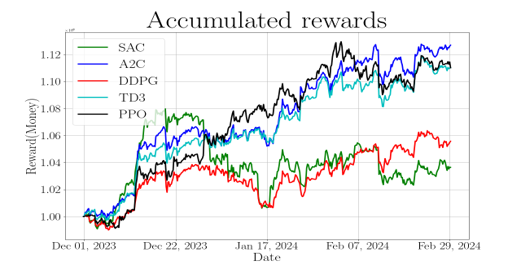
\includegraphics[width=.6\textwidth]{figures/Accumulated_Rewards_Reference.png}
        \caption{Performance of Reinforcement Learning Strategies on Financial Asset Trading \cite{RLinFinance}}
        \label{fig:Accumulated_Rewards_Reference}
\end{figure}

\subsection{Buy/Sell/Hold Agent}\label{sec:Model_Design:Buy_Sell_Hold_Agent}

\subsubsection{BSH Action Space}\label{sec:Model_Design:Buy_Sell_Hold_Agent:BSH_Action_Space}

\begin{table}[hbt!]
        \centering
        \begin{tabular}{||c|c||}
                \hline
                \textbf{Action} & \textbf{Description} \\
                \hline
                \hline
                0 & Invested in cash. \\
                \hline
                1 & Invested in asset. \\
                \hline
        \end{tabular}
        \caption{Buy/Sell/Hold Agent Action Space}
        \label{tab:Buy_Sell_Hold_Agent_Action_Space}
\end{table}

\begin{figure}[hbt!]
        \centering
        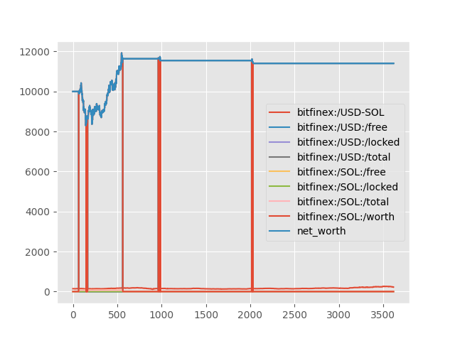
\includegraphics[width=.6\textwidth]{figures/BSH_Action_Example.png}
        \caption{BSH Action Plot Example}
        \label{fig:Limit Order Action Plot Example}
\end{figure}

\subsubsection{Position-Based Reward Function}\label{sec:Model_Design:Buy_Sell_Hold_Agent:Position_Based_Reward_Function}

\begin{equation}\label{eq:Position_Based_Reward_Function}
        R_t = \left(\text{Close}_{t} - \text{Close}_{t-1}\right) \cdot x_t
\end{equation}

\subsection{Managed Risk Agent}\label{sec:Model_Design:Managed_Risk_Agent}

\subsubsection{Limit Order Action Space}\label{sec:Model_Design:Managed_Risk_Agent:Limit_Order_Action_Space}

\begin{table}[hbt!]
        \centering
        \begin{tabular}{||c|c|c||}
                \hline
                \textbf{Action Parameter} & \textbf{Description} & \textbf{Values used} \\
                \hline
                \hline
                Stop Loss & Maximum loss before selling & [$2\%$, $5\%$, $10\%$] \\
                \hline
                Take Profit & Maximum profit before selling. & [$1\%$, $5\%$, $10\%$, $15\%$] \\
                \hline
                Trade Size & Size of next trade. & [$\frac{1}{16}$, $\frac{2}{16}$, \dots, $1$]\\
                \hline
        \end{tabular}
        \caption{Limit Order Agent Action Space}
        \label{tab:Limit_Order_Agent_Action_Space}
\end{table}

\begin{figure}[hbt!]
        \centering
        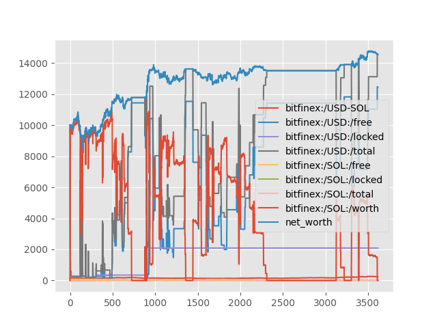
\includegraphics[width=.6\textwidth]{figures/Risk_action_example.png}
        \caption{Limit Order Action Plot Example}
        \label{fig:Limit Order Action Plot Example}
\end{figure}

\subsubsection{Sortino Ratio Reward Function}\label{sec:Model_Design:Managed_Risk_Agent:Sortino_Ratio_Reward_Function}

\cite{sortino1994performance}

\begin{equation}\label{eq:Sortino_Ratio_Reward_Function}
        R_t = \frac{\frac{x_{t} - x_{t-1}}{x_{t-1}} - r_f}{\sigma_d}
\end{equation}

\section{Implementation}\label{sec:Implementation}
The models described above were implemented in Python by leveraging third party libraries shown in table \ref{tab:3rd_Party_Libraries}.
The hyperparameters for the technical analysis indicators are shown in table \ref{tab:Technical_Analysis_Indicator_Hyperparameters}.

\begin{table}[hbt!]
        \centering
        \begin{tabular}{||c|c|c|c||}
                \hline
                \textbf{Technical Analysis Indicator} & \textbf{Hyperparameters} & \textbf{Target Asset} & \textbf{Related Asset(s)} \\
                \hline
                \hline
                Relative Strength Index & $k=14$ & \checkmark & \checkmark \\
                \hline
                Consumer Commodity Index & $k=30$ & \checkmark & \\
                \hline
                Average Directional index & $k=30$ & \checkmark & \\
                \hline
                Simple Moving Average & $k=30$ & \checkmark & \\
                \hline
                Simple Moving Average & $k=60$ & \checkmark & \\
                \hline
                Moving Average Convergence/Divergence & $fast=12, slow=26$ & \checkmark & \checkmark \\
                \hline
                Bollinger Bands & $k=20$ & \checkmark & \\
                \hline
                Average True Range & $k=20$ & \checkmark & \\
                \hline
                Rate of Change & $k=20$ & \checkmark & \\
                \hline
                On-Balance Volume & $k=20$ & \checkmark & \\
                \hline
                Stochastic Oscillator & $k=20$ & \checkmark & \\
                \hline
        \end{tabular}
        \caption{Technical Analysis Indicator Hyperparameters}
        \label{tab:Technical_Analysis_Indicator_Hyperparameters}
\end{table}

\begin{table}[hbt!]
        \centering
        \begin{tabular}{|c|c|}
                \hline
                \textbf{3rd Party Libraries} & \textbf{Usage} \\
                \hline
                \hline
                NumPy \cite{harris2020array} & \\
                \hline
                pandas \cite{reback2020pandas} & \\
                \hline
                pandas\_ta \cite{pandas-ta} & \\
                \hline
                TensorTrade \cite{Tensortrade} & \\
                \hline
                stable\_baselines3 \cite{stable-baselines3} & \\
                \hline
        \end{tabular}
        \caption{3rd Party Libraries}
        \label{tab:3rd_Party_Libraries}
\end{table}

\section{Analysis}\label{sec:Analysis}

\begin{figure}[hbt!]
        \centering
        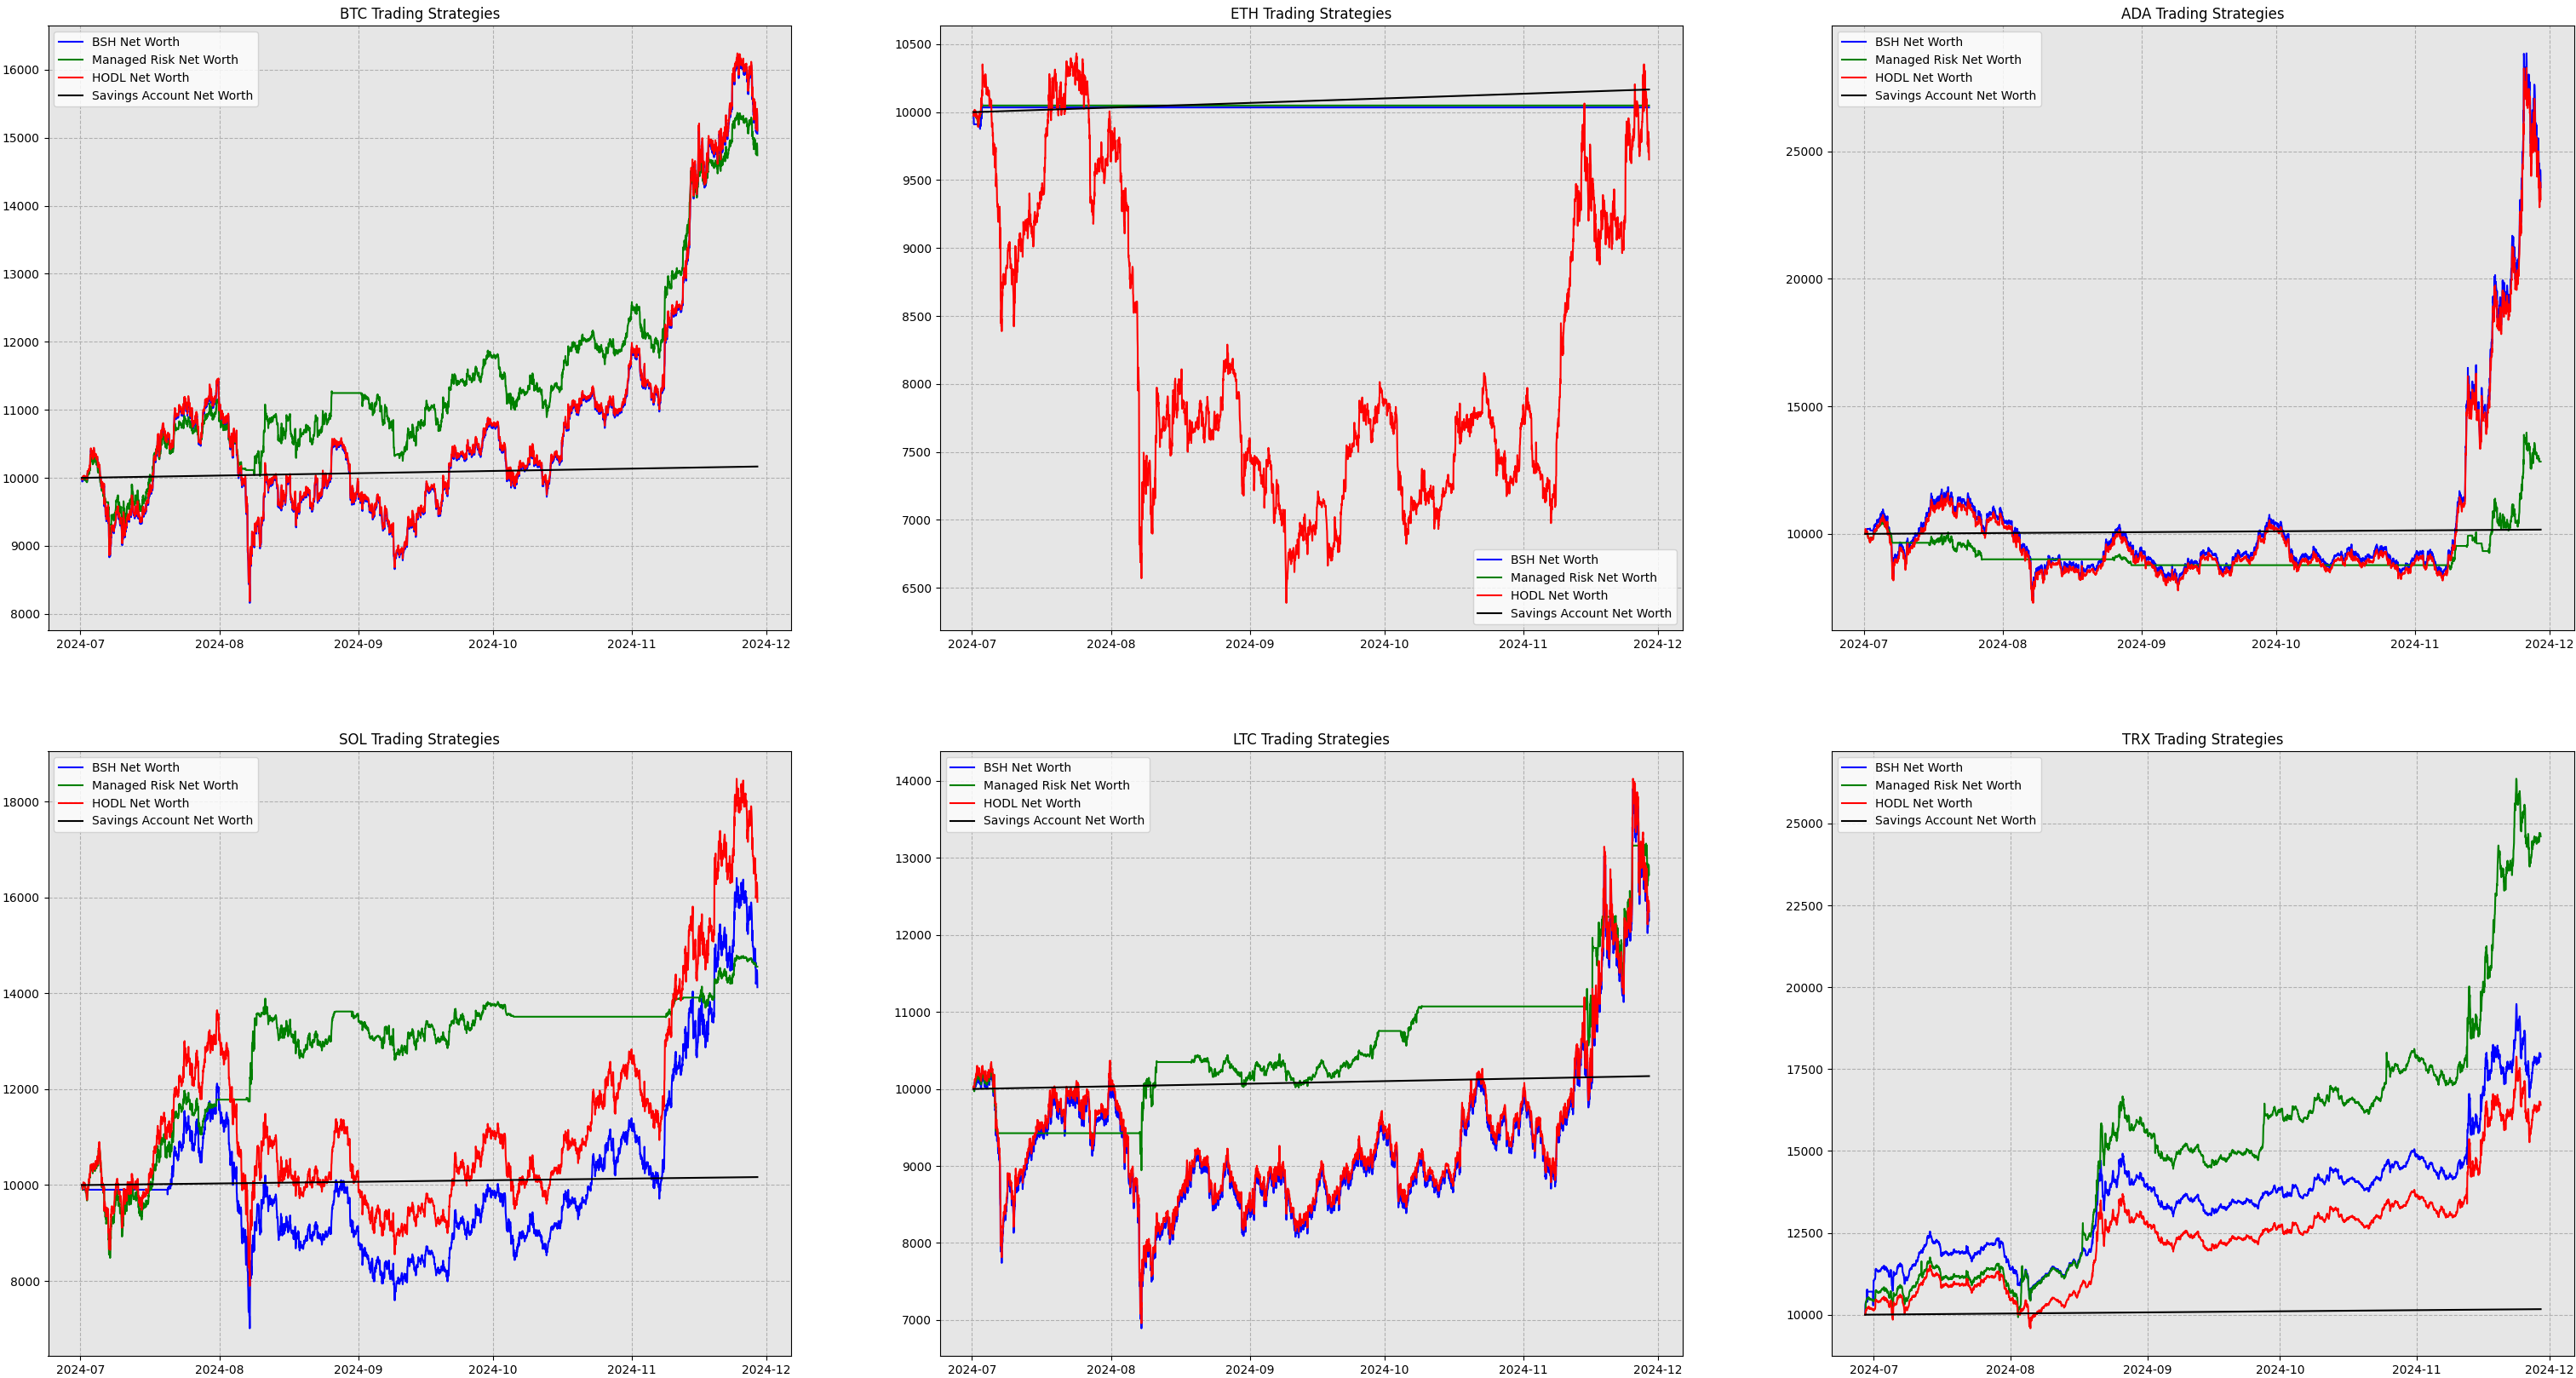
\includegraphics[width=\textwidth]{figures/model_results_per_asset.png}
        \caption{Results by Cryptocurrency}
        \label{fig:Aggregate Results}
\end{figure}

\begin{figure}[hbt!]
        \centering
        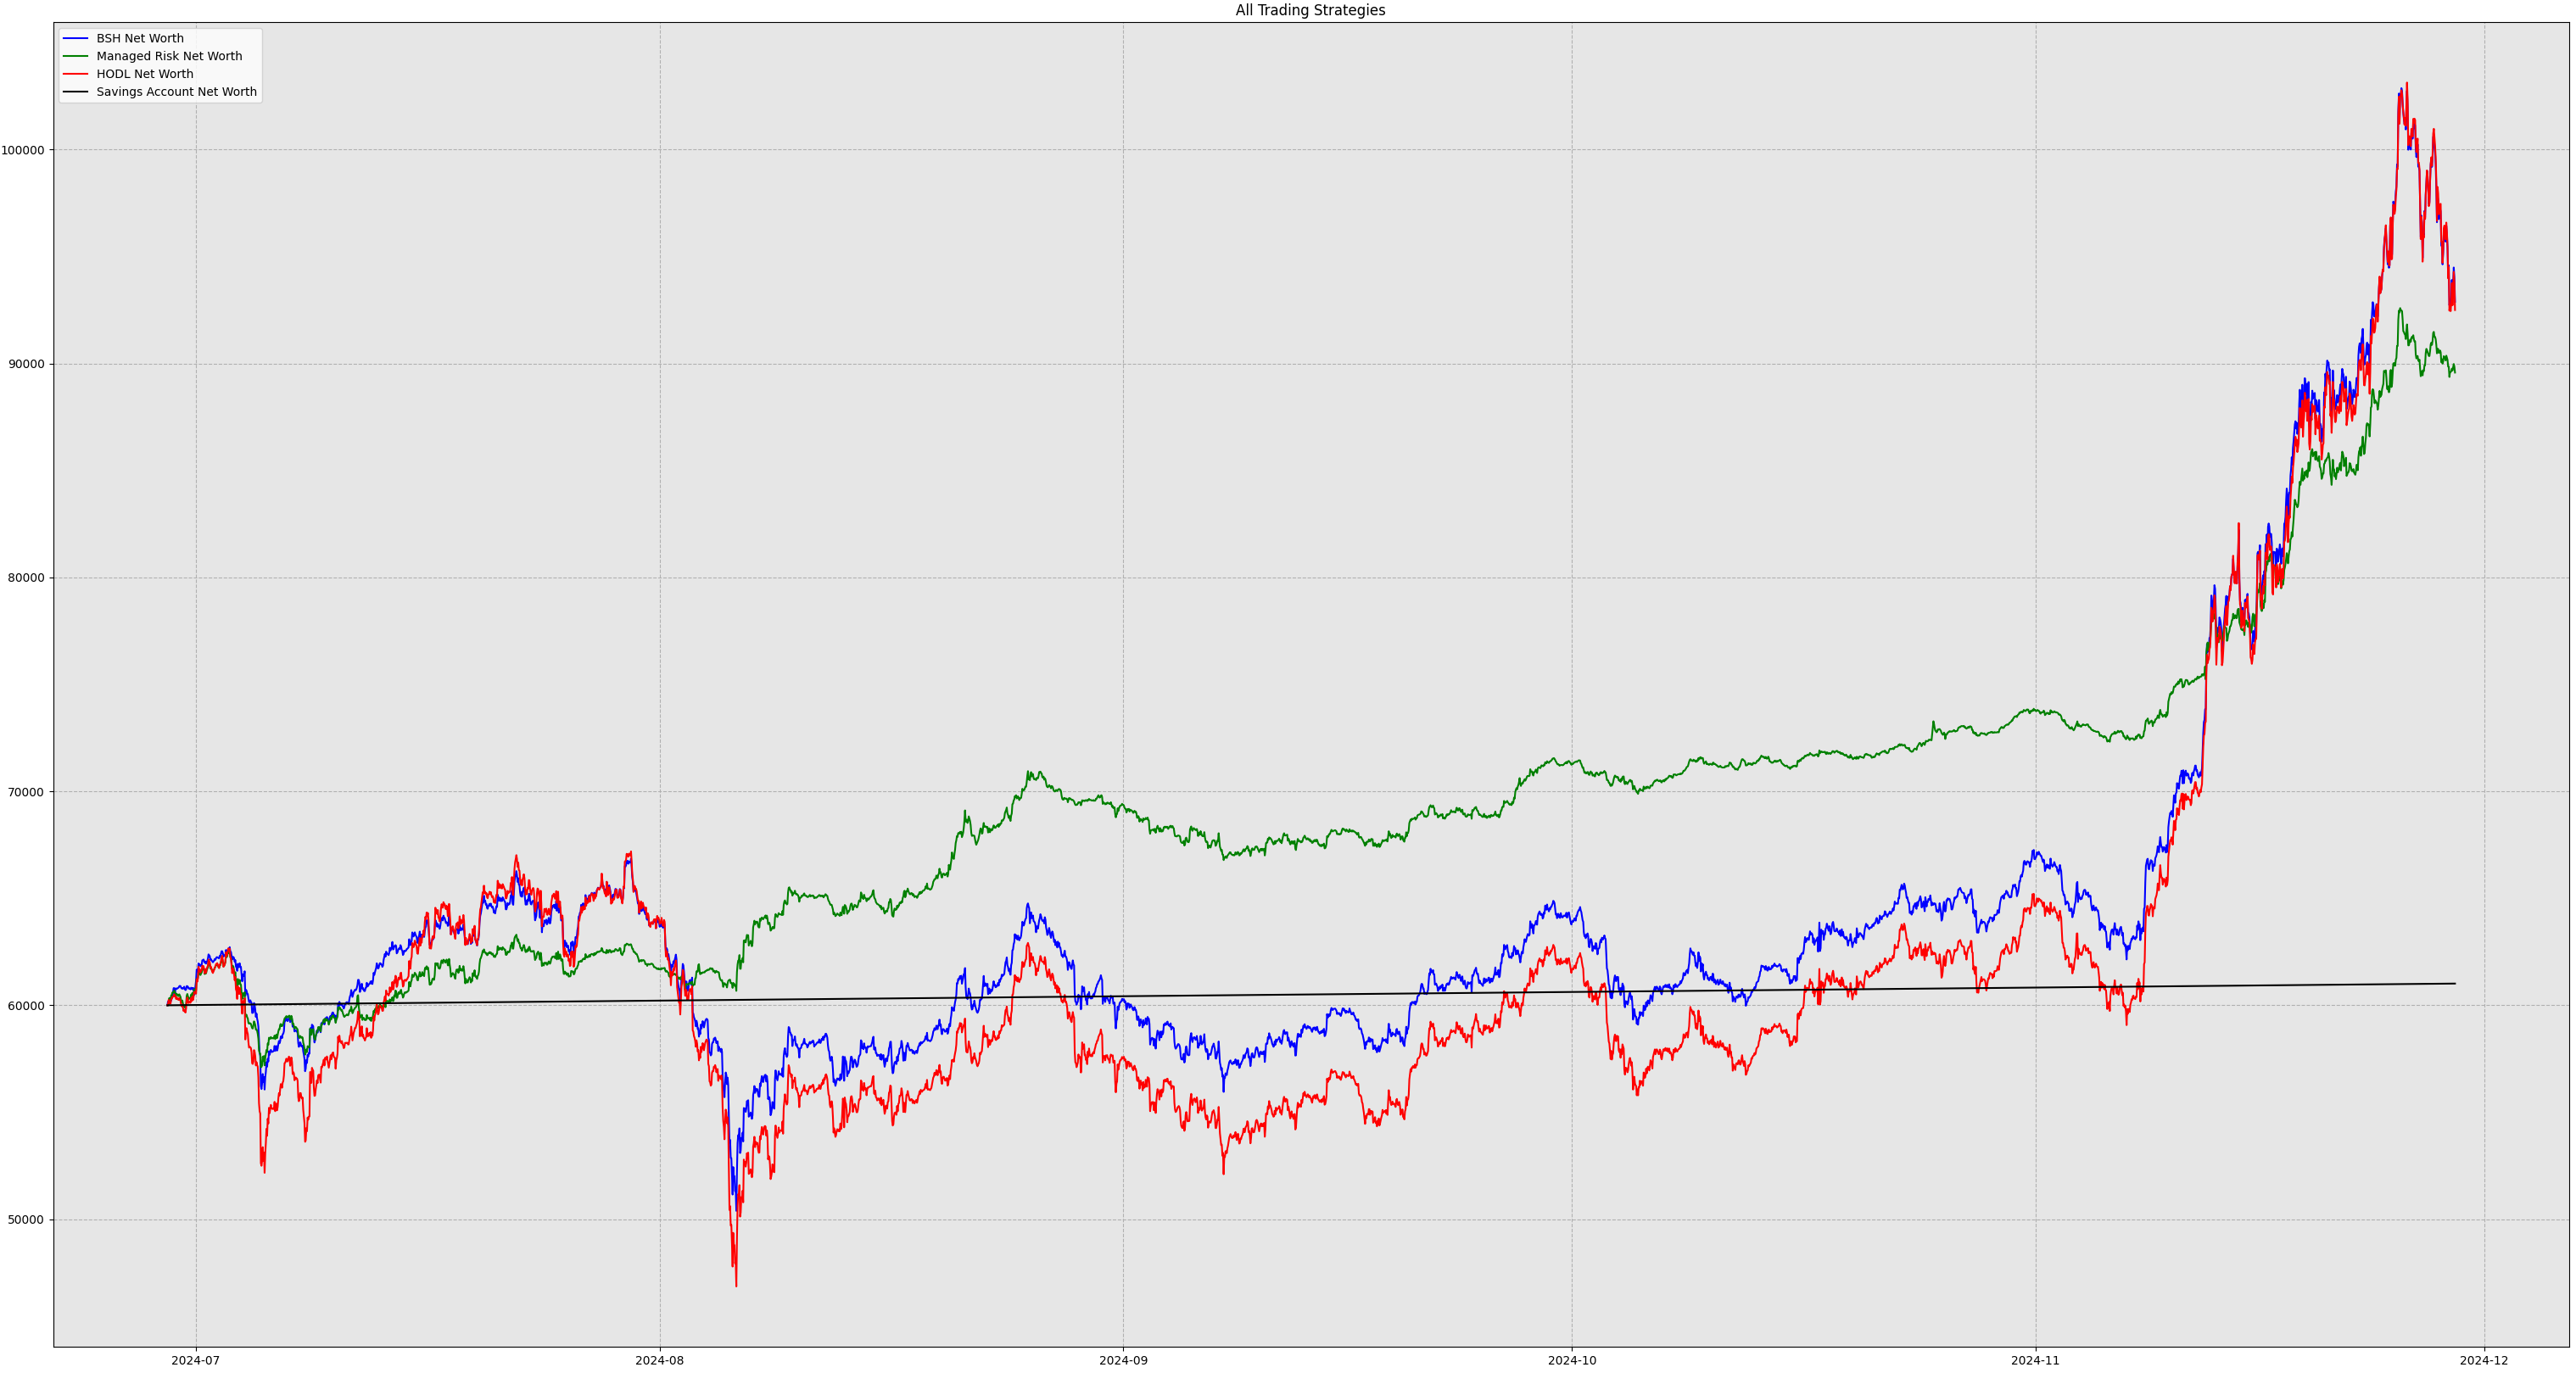
\includegraphics[width=\textwidth]{figures/aggregate_model_results.png}
        \caption{Aggregate Results}
        \label{fig:Aggregate Results}
\end{figure}

\section{Discussion}\label{sec:Discussion}

\section{Future Work}\label{sec:Future_Work}

\section*{Appendix}\label{sec:Appendix}

\section*{Acknowledgements}\label{sec:Acknowledgements}

\bibliography{pavlovBib}

\end{document}